\documentclass{vldb}
\usepackage{graphicx}
\usepackage{balance} 

\begin{document}


\section{Introduction}

TODO: generalize intro (not only plot)

\par The International Movie Database (IMDb) with its over 3 million listed titles provides a great resources for information about all sorts of movies. Maintaining this amount of data is quite challenging as new movies need to be added all the time.
Although the data is in a multi GB space one would not necessarily consider it to be ‘Big Data’. Especially in comparison to things like Twitters continuous stream of data or even large scale sensor networks the IMDb is quite small and any analysis could probably be done with conventional systems. But for this academic project we wanted to try to build a scaleable solution, which could be easily adopted for other, larger data sources.

\par For this project we decided to try a classification task on the available movie metadata to predict its genres. This could be helpful for people who enter information about new movies or also to complete the IMDb since there are about 300.000 movies without genre information.
Part of this analysis it text classification which is a problem that occurs in many domains.

\par For the genre classification it is also interesting whether it is possible to predict a genre in a reliable way. Often this task is challenging even for humans cause a genre itself doesn’t have formal specification and can be a bit fuzzy. There are also mixups of genres, like a tragic comedy, which might be hard to classify since they contain features of multiple genres. Evaluating whether a machine can learn sort of a formal definition in form of some model is interesting since a further analysis of the model could lead to formal, human understandable definition of a genre. It could solve the question of “What makes up a genre?”.



\section{Problem Statement}
\subsection{Background}
Movie genres are manually created categorical labels to characterize different movies. These genre labels can be used to describe the movie, contribute in movie recommendation based on the domain specified interests and some other fields. Currently the movie genres annotation are determined by us. The complexity in automatic genre classification is caused by the fact that usually the genres are not well  defined. Normally there are no strict definitions or boundaries between 2 different genres.  And of cause they share certain overlapping characteristics.
\par Facing the fact that the number of movie is growing at a fast pace, automatic movie genres classification can assist or replace the human work in this process and provide important component for the complete movie information and in addition, structure the movie based on the genres. Thus, we begin to think about: what kind of information is sufficient to automatically classify the movie and how to approach that?
\par After considering our requirement and all the related movie information component, We decide to focus on building a scalable movie genre classification system based on their plot description. 

\subsection{Dataset} 
Dataset:The dataset we use is the publicly available data from the Internet Movie Database(IMDb). IMDb is an online dataset which provides information related to movies, television programs and video games. The information includes actors, production crew and fictional characters featured in these. There are some publicly available datasets containing a subset of the online database, which can be downloaded and processed. 
\par The dataset is organized into a set of compressed text files, where each file contains information on a specific aspect. The files we use are the plot.list and genres.list files and the size is more than 400MB. It contains all the plot description, genre information we need and is big enough to test the scalability.
\subsection{Tools}
\par Python: Python is a fast and friendly language. It’s easy to learn and can work everywhere. The raw data from IMDb can not be used directly, so we choose Python to do the preprocessing work and generate processed data for the next steps.
\par Apache Spark: Spark is an open source Apache project built around speed, ease of use. It provides a faster and more general data processing platform. Spark enables we to quickly write applications in Java, Scala, or Python. It comes with a built-in set of over 80 high-level operators. And we can use it interactively to query data within the shell. Other than Spark Core API, there are additional libraries that are part of the Spark ecosystem and provide additional capabilities in Big Data analytics and Machine Learning areas. The scalable machine learning library consisting of common learning algorithms and utilities, including classification, regression, clustering, collaborative filtering, dimensionality reduction, as well as underlying optimization primitives.

\section{Methodology}
\subsection{Apache Spark Pipeline}
In machine learning, it is common to run a sequence of algorithms to process and learn from the data, a regular text document processing workflow might include several steps like:
\begin{itemize}
\item {Split the document into words.}
\item {Convert each document's words into a numerical feature vector.}
\item {Learn a prediction model using the feature vectors and labels.}
\end{itemize}
\par Spark ML represents such a workflow as a Pipeline, which consists of a sequence of PipelineStages (each stage is either a Transformer or an Estimator) to be run in a specific order. The input dataset is modified as it passes through each stage. For Transformer stages, the transform() method is called on the dataset. For Estimator stages, the fit() method is called to produce a Transformer (which becomes part of the PipelineModel, or fitted Pipeline), and that Transformer’s transform() method is called on the dataset.
\par This figure shows the 3-stage pipeline we used in the project. These 3 stages are all transformers.  Each stage’s transform() method updates the dataset and passes it to the next stage. The bottom row represents data flowing through the pipeline, where cylinders indicate DataFrames. The Tokenizer.transform() method splits the raw text documents into words, adding a new column with words into the dataset. The HashingTF.transform() and idf.transform() method converts the words column into feature vectors, adding a new column with those vectors to the dataset. Then SVM.train() is called to produce a SVMModel. After that the pipeline calls SVM.predict() method on the dataset and predict the result.
\begin{figure}
\begin{center}
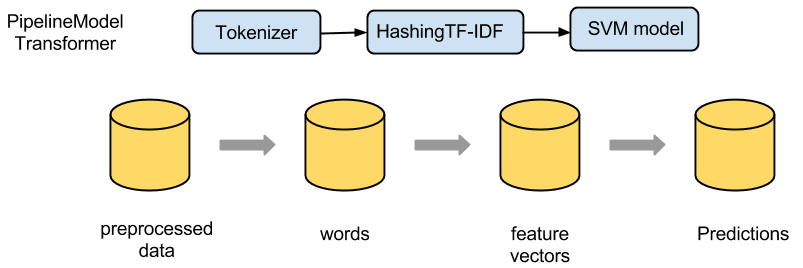
\includegraphics[width=3.50in]{AIM3-pipeline.png}
\caption{movie genres classification pipeline}
\end{center}
\end{figure}
\subsection{Preprocessing}
\par To get start, we first use Tableau to get a insight of the dataset. 
\begin{figure}
\begin{center}
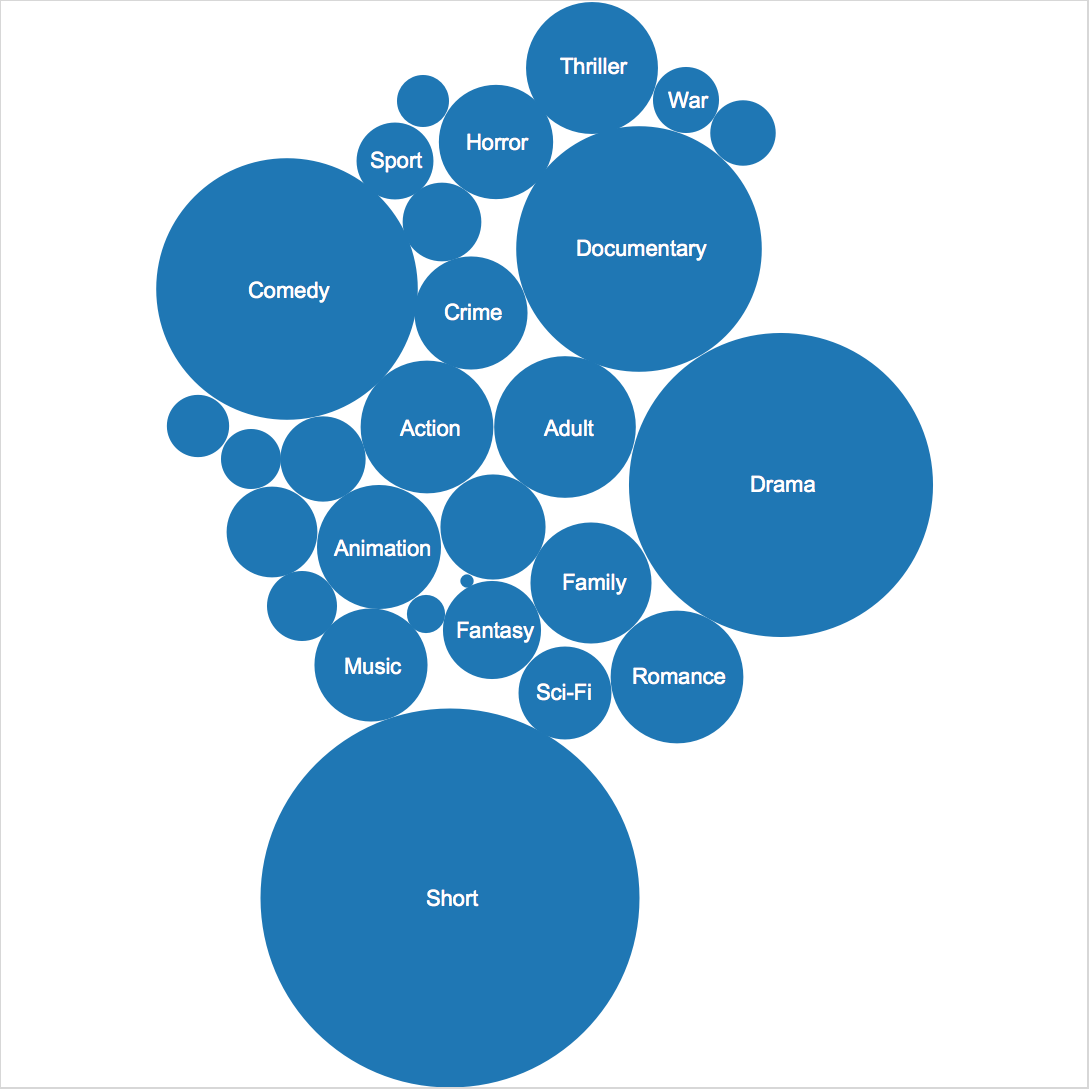
\includegraphics[width=3.00in]{tableau.png}
\caption{insight of the data using Tableau}
\end{center}
\end{figure}
\subsection{Feature Extraction}
Term frequency-inverse document frequency (TF-IDF) is a feature vectorization method that is intended to reflect how important a word is to a document in a collection of the corpus. The tf-idf value increases probability to the number of times a word appears in the document, but is offset by the frequency of the word in the corpus, which helps to adjust for the fact that some words appear more frequently in general.
\par Denote a term by $t$, a document by $d$, and the corpus by $D$. Term frequency $TF(t,d)$ is the number of times term $t$ appears in document $d$, while the document frequency $DF(t,D)$ is the number of documents that contain term $t$ in corpus $D$. However, if we only use term frequency, for some common words, like "the", it will tend to incorrectly emphasize the documents which happen to use "the" more frequently. But these kind of words can't provide enough information to distinguish relevant and non-relevant documents and terms. If a term appears very often across the corpus, it means it doesn’t carry special information about a particular document. Thus, we use inverse document frequency, a numerical measure to show how much information a term carries:
\begin{displaymath}
IDF(t,D) = \log\frac{|D|+1}{DF(t,D)+1},
\end{displaymath}
where $|D|$ is the number of documents in the corpus. Since logarithm is used, if a term appears in all documents, its $IDF$ value becomes 0. Note that a smoothing term is applied to avoid dividing by zero for terms outside the corpus. The TF-IDF measure is simply the product of $TF$ and $IDF$:
\begin{displaymath}
TFIDF(t,d,D)=TF(t,d)⋅IDF(t,D).
\end{displaymath} 
\par Also, in the implementation of TF-IDF of in  Apache Spark machine learning library, raw feature is mapped into an index(term) by using a hashing function. Then term frequency is calculated based on the mapped indices. This approach avoids the need to compute a global term-to-index map, which can be expensive for a large corpus, but it suffers from potential hash collisions, where different raw features may become the same term after hashing. To reduce the chance of collision, we can increase the target feature dimension, i.e., the number of buckets of the hash table. The default feature dimension is $2^{20}=1048576$
\par By using tf-idf, we generate a vector for every plot description.

\subsection{Classification}
In machine learning, support vector machines(SVMs) are supervised learning models used for classification and regression analysis. Given a set of training examples, each marked for belonging to one of two categories, an SVM training algorithm builds a model that assigns new examples into one category or the other, making it a non-probabilistic binary linear classifier. 
\par An SVM model constructs a hyperplane in high(or infinite)dimensional space, which can be used for classification, regression, or other tasks. Intuitively, a good separation is achieved by the hyperplane that has the largest distance to the nearest training-data point of any class (so-called functional margin), since in general the larger the margin the lower the generalization error of the classifier.
\par Given some training dataset $\mathcal{D}$ containing $n$ points:
\begin{displaymath}
\mathcal{D} = \{(\mathbf{x}_i,y_i)|\mathbf{x}_i \in \mathbb{R}^p,y_i\in\{-1,1\}\}^n _{i=1}
\end{displaymath}
where $y_i$ is either $1$ or $-1$, indicating the class to which $\mathbf{x}_i$ belongs. Each $\mathbf{x}_i$ is a $p$ dimentional vector. If the data is linealy seperable, we can find a hyperplane:
\begin{displaymath}
\mathbf{w}\cdot\mathbf{x}-b=0 
\end{displaymath}
to seperate the dataset and by determin the distance from the data point to the hyperplane $|\mathbf{w}\cdot\mathbf{x}+b|$ is positive or negative to see which class this pint belongs to.

\par  To find the maximum margin to divide the dataset into 2 classes($y=1$ or $y=-1$), we can select two hyperplanes in a way that they separate the data and there are no points between them, and then try to maximize their distance. The region bounded by them is called "the margin". These hyperplanes can be described by the equations
\begin{displaymath}
\mathbf{w}\cdot\mathbf{x}-b=1
\end{displaymath}
and
\begin{displaymath}
\mathbf{w}\cdot\mathbf{x}-b=-1
\end{displaymath}
\begin{figure}
\begin{center}
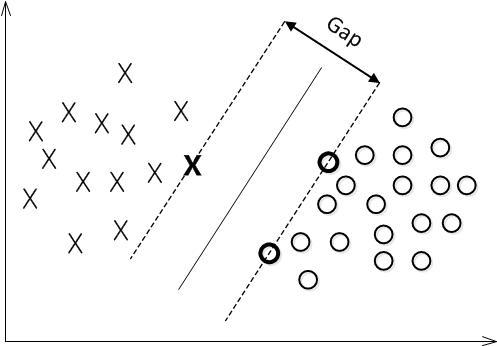
\includegraphics[width=2.50in]{SVM.jpeg}
\caption{margins for an SVM trained with samples from two classes}
\end{center}
\end{figure}
\par By using geometry, we find the distance between these two hyperplanes is $\frac{2}{||w||}$, so we want to minimize $||w||$. As we also have to prevent data points from falling into the margin, we add the following constraint:
\begin{displaymath}
\begin{cases}
\mathbf{w}\cdot\mathbf{x}-b\ge1,y_i=1\\
\mathbf{w}\cdot\mathbf{x}-b\le-1,y_1=-1\\
\end{cases}
\end{displaymath}
This can be written as:
\begin{displaymath}
y_i(\mathbf{w}\cdot\mathbf{x}_i-b)\ge1,1\le i \le n
\end{displaymath}
\par More clearly, the constraint problem can be written as:
\begin{displaymath}
\arg\min\frac{1}{2}||\mathbf{w}||^2
\end{displaymath}
subject to (for any $i = 1,...,n$)
\begin{displaymath}
y_i(\mathbf{w}\cdot\mathbf{x}_i-b)\ge1
\end{displaymath}
After getting the $\mathbf{w}$, given a new data point, denoted by $\mathbf{x}$


\section{Experiment}

\par We started our experiments with using the plot descriptions and performed multiple runs with different number of learning iterations of the SVMs. After that we used other features of the movie to see whether we could do better. We also combined several features.

\par The first approach was to use the plot description and transform it to a TF-IDF vector for each movie. For this approach we could use TODO movies, which had a plot description as well as a genre label. 

\par The second approach was to use keywords of the movies, which were explicitly assigned by the maintainers of the IMDb. This provides us a similar textual representation of the content of the movie but with the advantage of being already filtered by a human and also containing words that do not appear in a typical plot description but might describe the type of the movie quite well. We didn’t need to perform a TF-IDF transformation here since each keyword only appears once and we just constructed a vector per movie containing a 1 if it has a certain keyword and 0 if not. With this approach we could use TODO movies, which provided a set of keywords and a genre label.

\par The third approach was to create a connection between actors and the genre of movies they usually appear in. This feature isn’t content based at all but could be of significance cause we assume that most actors stick to one kind of genre during their carer. Similar to the keywords approach we didn’t use a TF-IDF transformation and just binary n-dimensional vector to represent the fact whether a actor appeared in the movie or not. Here we had a dataset of TODO movies, which provided a list of actors as well as a genre label.

\par As a final experiment we combined all 3 features. Therefore we constructed a set of 3 feature vectors - one for plot, one for keywords and one for actors - per movie. Now we trained 3 SVMs per genre - one for each feature vector. In the testing phase we feed the feature vectors to the SVMs and build a simple average over the results of all 3 SVMs per genre. Cause we could only use movies which provide valid feature vectors for all 3 features, we could only use a dataset of TODO movies.

\par For all experiments we tried to classify the movie in 24 genres (see graph TODO). We didn’t consider the genre “Short” in our computation and analysis since it’s a very large and fuzzy genre which is basically only based on the length of a movie but the goal was to create a content related classification. Also the “genre” TODO only had one(?) movie in it was omitted cause of that.

TODO: numbers and graph for \#movies with features



\section{Results}

TODO: explain “story”
TODO: mention different data set sizes per feature/feature combination -> impact on results
TODO: insert graphs

\par Using the plot description as the only feature wasn’t really successful. Although the portion of erroneous single classification operations was at around 6 \%, there were many movies which weren’t classified correctly. This is caused by the fact that we use 24 SVMs - one SVM for each genre. Most of these SVMs answer with a correct prediction - in most cases with “false”, cause a movie usually only belongs to 1 to 3 genres. But it is enough that one of those SVMs answers with a wrong value and the movie ends up misclassified.
\par Another interesting observation is that the amount of errors for the genres Drama, Comedy and Documentary is significantly higher than for other genres. Those 3 genres are the most common ones. One could expect that the SVMs are trained more precisely cause of a larger amount of positive training examples and a therefore more even distribution of negative and positive data points. But it seems like that the larger amount of movies in those genres leads to more diverse plot descriptions and a more fuzzy definition of the genre.
\par When looking at the development of false-positive and false-negative classifications over increasing number of training iterations, one can see an overfitting of the model for Drama in alternating directions. With 5 iterations the false-positive rate is low and the false-negative rate is high, for 20 iterations the false-positive rate is high and the false-negative rate is low. The gap and error rate reduces with increasing number of training iterations but continues to be visible even at around 100 iterations.
\par For most of the other genres false-positives aren’t an issue until 10 to 15 or even until 35 iterations. This is most likely due to the small amount of positive training examples which leads to strong tendency of always answering with no.
\par The false-negative rates are quite stable with in most cases a slight tendency to a lower error rate, but there are also some genres like Romance which have a constant increase in the error rate with increasing number of iterations. The most significant improvements can be seen between 0 and 25 iterations.
\par If we look at the overall error rate there’s usually an improvement with increasing number of training iterations. It seems to be stable after around 50 iterations. An reduction of false-negatives is often consumed by an increase in false-positives, leading to nearly horizontal lines for some genres. The alternating false-negatives and false-positives for genres like Drama or Comedy even themselves out and lead to a continuous curve in the total error rate.
\par The number of completely correctly classified movies increased nearly continuously with increasing number of iterations - as one would expect it to be after seeing decreasing error rates. Interestingly there are small drops in the curve at 15 and 25 iterations. Those are the same spots where the Drama false-negative rates are high but the Drama false-positive rates are low. The curve increases significantly until 30 iterations with 23.7 \% accuracy and only slowly develops to 25 \% accuracy at 100 iterations.
\par Overall the approach wasn’t satisfying with only ~25 \% completely correctly classified movies and in general the following rules hold:
\begin{itemize}
\item {The more SVMs iterations the more precise is the classification.}
\item {The more movies belong to a genre the more errors in classification will happen.}
\item {For reasonable results one can stop training after around 50 iterations.}
\end{itemize}


\bigskip
\par In the next experiment we used the keywords as the only feature. The overall result was slightly better with 27.8 \% to 29.6 \% completely correctly classified movies.
As for the plot based classification the genres Drama, Comedy and Documentary were the most difficult to classify. With false-positive rates of 13 to 19 \%. All other genres had false-positives rates below 7 \%. Interestingly the false-positive rate for Comedy was about five percent points higher than Drama, whereas the false-negative rate of Drama was around 10 \% while the false-negative rate for Comedy and Documentary weren’t much above the lower than 1 \% rates of the other genres. Overall the false-negative rates were really small and much better than for the plot based classification. For a higher number of iterations the same issue if increasing false-negatives rates were observable. The phenomena of alternating high and low false-negative and false-positive rates couldn’t be observed.
\par In the overall error rates Drama was the most difficult to classify (~24 \% error) followed by Comedy (TODO) and documentary(TODO). All other genres where quite close and below TODO \% error rate. The error rate and also the rate of completely correctly classified movies did’t improve significantly with increasing number of iterations. Again most improvements in false-positives rates were neutralised by increasing false-negative rates. Only a small improvement between 5 and 20 iterations was noteable. The most improvements were observable for the 3 difficult genres Drama, Comedy \& Documentary.

\bigskip
\par The third experiment was to to only use the actors data as the feature vector. This experiment did’t perform much better than the plot based classification and lead to nearly the same rate of completely correctly classified movies of about 24.8 \%.
\par The error rates stayed nearly constant and also the rate of completely correctly classified movies didn’t change with an increasing number of training iterations. Cause of that this approach delivered better results for a low number of iterations and was faster in the training phase cause of a lower dimensionality of the feature vectors.
As in the previous two experiments the genres Drama, Comedy and Documentary were the ones with the highest error rates.

\bigskip
All 3 combined:
significantly better results (up to 43,9%)
significant increase with iterations (23,9% -> 43,9%)
only small drops in between (at 20, after 45 and at 70 iterations)
largest increase between 5 and 15 iterations
very long training phase (~ 3 times the time cause 3 SVMs)
TODO: look at false pos / false neg rates

\section{Conclusion}

combination of features is better
more SVM training doesn’t provide always better results -> time/cost vs precision gain
quality of the data might differ -> huge impact
future work: more fetaures, try different feature combinations, filter for only relevant/high quality movies/data
Spark provides nice interface and ML lib -> easy to use

\section{Reference}


\end{document}
